\onehalfspacing
\section{Đề số 19}
\graphicspath{{./img/}}
\begin{bt} 
    \hfil
    \begin{enumerate}[a.]
        \item Tính giá trị biểu thức $A=\left(2 \frac{1}{3}+3,5\right):\left(-4 \frac{1}{6}+3 \frac{1}{7}\right)+7,5$
        \item Rút gọn biểu thức: $\quad B=\frac{2 \cdot 8^4 \cdot 27^2+4 \cdot 6^9}{2^7 \cdot 6^7+2^7 \cdot 40 \cdot 9^4}$
        \item Tìm đa thức $M$ biết rằng: $M+\left(5 x^2-2 x y\right)=6 x^2+9 x y-y^2$.
        Tính giá trị của M khi $x$, $y$ thỏa mãn $(2 x-5)^{2012}+(3 y+4)^{2014} \leq 0$.
    \end{enumerate}
\loigiai{
    \begin{enumerate}
        \item Ta có:
        $A =\left(2 \frac{1}{3}+3,5\right):\left(-4 \frac{1}{6}+3 \frac{1}{7}\right)+7,5=\left(\frac{7}{3}+\frac{7}{2}\right):\left(\frac{-25}{6}+\frac{22}{7}\right)+\frac{15}{2} \\[5px]
        =\frac{35}{6}: \frac{-43}{42}+\frac{15}{2}=\frac{-245}{43}+\frac{15}{2}=\frac{-490}{86}+\frac{645}{86}=\frac{155}{86}$\\[5px]
        \item Ta có:\\[5px]
        $B =\frac{2 \times 8^4 \times 27^2+4 \times 6^9}{2^7 \times 6^7+2^7 \times 40 \times 9^4}=\frac{2^{13} \times 3^6+2^{11} \times 3^9}{2^{14} \times 3^7+2^{10} \times 3^8 \times 5} \\[5px]
        =\frac{2^{11} \times 3^6 \times\left(2^2+3^3\right)}{2^{10} \times 3^7 \times\left(2^4+3 \times 5\right)}=\frac{2}{3}$
        \item Ta có:\\[5px]
        $M+\left(5 x^2-2 x y\right)=6 x^2+9 x y-y^2=>M=6 x^2+9 x y-y^2-\left(5 x^2-2 x y\right) \\[5px]
        \Rightarrow M=6 x^2+9 x y-y^2-5 x^2+2 x y=x^2+11 x y-y^2 \\[5px]
        \text { Ta có }(2 x-5)^{2012}+(3 y+4)^{2014} \leq 0 \\[5px]
        \text { Ta có : }\left\{\begin{array}{l}
        (2 x-5)^{2012} \geq 0 \\[5px]
        (3 y+4)^{2014} \geq 0
        \end{array}=>(2 x-5)^{2012}+(3 y+4)^{2014} \geq 0\right.$\\[5px]
        $\text { Mà }(2 x-5)^{2012}+(3 y+4)^{2014} \leq 0 \Rightarrow(2 x-5)^{2012}+(3 y+4)^{2014}=0$\\[5px]
        $\Rightarrow\left\{\begin{array} { l } 
{ ( 2 x - 5 ) ^ { 2 0 1 2 } = 0 } \\[5px]
{ ( 3 y + 4 ) ^ { 2 0 1 4 } = 0 }
        \end{array} \Rightarrow \left\{\begin{array} { l } 
        { x = 2 \frac { 1 } { 2 } } \\[5px]
        { y = - 1 \frac { 1 } { 3 } }
        \end{array} . \\[5px]
        \text { Vậy } \left\{\begin{array}{l}
        x=2 \frac{1}{2} \\[5px]
        y=-1 \frac{1}{3}
        \end{array}\right.\right.\right.$\\[5px]
        Vậy $M=\left(\frac{5}{2}\right)^2+11 \times \frac{5}{2} \times\left(-\frac{4}{3}\right)-\left(\frac{-4}{3}\right)^2=\frac{25}{4}-\frac{110}{3}-\frac{16}{9}=\frac{-1159}{36}$
    \end{enumerate}
}
\end{bt}

\begin{bt}
    \hfill
	\begin{enumerate}[a.]
        \item $\operatorname{Tim} x: \frac{1}{2}-\left|x+\frac{1}{5}\right|=\frac{1}{3}$
        \item Tìm $\mathrm{x}, \mathrm{y}, \mathrm{z}$ biết: $2 x=3 y ; 4 y=5 z$ và $x+y+z=11$
        \item Tìm $x$, biết : $(x+2)^{n+1}=(x+2)^{n+11}$ (Với $\mathrm{n}$ là số tự nhiên)
    \end{enumerate}
	\loigiai{
        \begin{enumerate}
            \item Ta có: $\frac{1}{2}-\left|\mathrm{x}+\frac{1}{5}\right|=\frac{1}{3} \Leftrightarrow\left|x+\frac{1}{5}\right|=\frac{1}{2}-\frac{1}{3}\\[5px] \Leftrightarrow\left|x+\frac{1}{5}\right|=\frac{1}{6}$\\[5px]
            TH1: $\mathrm{x}+\frac{1}{5}=\frac{1}{6} \Rightarrow \mathrm{x}=-\frac{1}{30}$\\[5px]
            TH2: $x+\frac{1}{5}=-\frac{1}{6} \Rightarrow x=-\frac{1}{6}-\frac{1}{5}==-\frac{11}{30}$\\[5px]
            Vậy $x=-\frac{1}{30} ; x=-\frac{11}{30}$\\[5px]
            \item Ta có : $2 \mathrm{x}=3 \mathrm{y}$ suy ra $\frac{x}{3}=\frac{y}{2}$ hay $\frac{x}{15}=\frac{y}{10}$\\[5px]
            $4 \mathrm{y}=5 \mathrm{z} \text { suy ra } \frac{y}{5}=\frac{z}{4} \text { hay } \frac{y}{10}=\frac{z}{8}$\\[5px]
            Vậy $\frac{x}{15}=\frac{y}{10}=\frac{z}{8}$\\[5px]
            Theo tính chất dãy tỉ số bằng nhau:\\[5px]
            $\frac{x}{15}=\frac{y}{10}=\frac{z}{8}=\frac{x+y+z}{15+10+8}=\frac{11}{33}=\frac{1}{3}$\\[5px]
            Suy ra $x=5, y=\frac{10}{3}, z=\frac{8}{3}$
            \item $\text {Ta có: }(x+2)^{n+1}=(x+2)^{n+11} \\[5px]
                (x+2)^{n+1}-(x+2)^{n+11}=0 \\[5px]
                (x+2)^{n+1}\left[1-(x+2)^{10}\right]=0 \\[5px]
                \text { TH1: } (x+2)^{n+1}=0 \text { suy ra } x=-2 \\[5px]
                \text { TH2: } 1-(x+2)^{10}=0 \\[5px]
                \qquad \quad(x+2)^{10}=1 \\[5px]
                \quad x+2=1 \text { suy ra } x=-1 \\[5px]
                \quad x+2=-1 \text { suy ra } x=-3 \\[5px]
                \text { Vậy } x=-2 ; x=-1 ; x=-3$
        \end{enumerate}
    } 
\end{bt}

\begin{bt}
    \hfill
	\begin{enumerate}[a.]
        \item Tìm độ dài 3 cạnh của tam giác có chu vi bằng $13 \mathrm{~cm}$. Biết độ dài 3 đường cao tương ứng lân lượt là $2 \mathrm{~cm}, 3 \mathrm{~cm}, 4 \mathrm{~cm}$.
        \item Tìm $x, y$ nguyên biết: $2 x y-x-y=2$
    \end{enumerate}
	\loigiai{
        \begin{enumerate}
            \item Gọi độ dài ba cạnh của tam giác là $x, y, z(\mathrm{~cm})(x, y, z>0)$\\[5px]
            Theo bài ra ta có : $x+y+z=13$\\[5px]
            và $2 x=3 y=4 z=2 \mathrm{~S}_{\mathrm{ABC}}$\\[5px]
            Suy ra $\frac{x}{6}=\frac{y}{4}=\frac{z}{3}$\\[5px]
            Áp dụng tính chất dãy tỷ số bằng nhau\\[5px]
            $\frac{x}{6}=\frac{y}{4}=\frac{z}{3}=\frac{x+y+z}{6+4+3}=\frac{13}{13}=1 \\[5px]
            \text { suy ra } \mathrm{x}=6, \mathrm{y}=4 ; \mathrm{z}=3 \\[5px]
            \text { KL: } \mathrm{x}=6, \mathrm{y}=4, \mathrm{z}=3 \text {. }$
            \item Ta có: $2 x y-x-y=2$\\[5px]
            $4 x y-2 x-2 y=4 \\[5px]
            2 x(2 y-1)-2 y+1=5 \\[5px]
            (2 y-1)(2 x-1)=5$\\[5px]
            HS xét 4 trường hợp tìm ra $(x, y)=\{(1 ; 3) ;(3 ; 1) ;(-2 ; 0) ;(0 ;-2)\}$\\[5px]
            ( Mỗi trường hợp đúng cho 0.25 đ)\\[5px]
            Vậy $(x, y)=\{(1 ; 3) ;(3 ; 1) ;(-2 ; 0) ;(0 ;-2)\}$
        \end{enumerate}
    }
\end{bt}

\begin{bt}
    Cho tam giác $\mathrm{ABC}\left(\mathrm{AB}<\mathrm{AC}\right.$, góc $\left.\mathrm{B}=60^{\circ}\right)$. Hai phân giác $\mathrm{AD}$ và $\mathrm{CE}$ của $\triangle \mathrm{ABC}$ cắt nhau ở $\mathrm{I}$, từ trung điểm $\mathrm{M}$ của $\mathrm{BC}$ kẻ đường vuông góc với đường phân giác $\mathrm{AI}$ tại $\mathrm{H}$, cắt $\mathrm{AB}$ ở $\mathrm{P}$, cắt $\mathrm{AC}$ ở $\mathrm{K}$.
    \begin{enumerate}[a.]
        \item  Tính AIC
        \item Tính độ dài cạnh $\mathrm{AK}$ biết $P K=6 \mathrm{~cm}, A H=4 \mathrm{~cm}$.
        \item Chứng minh $\Delta$ IDE cân.
    \end{enumerate}
\loigiai{
    $$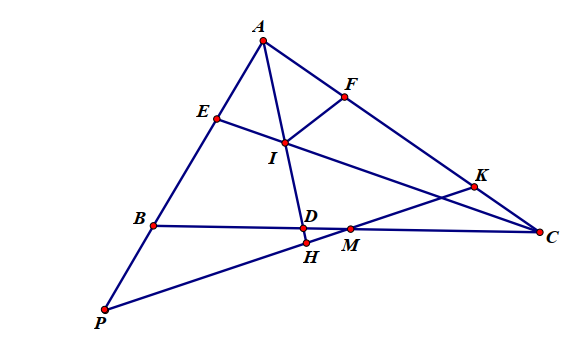
\includegraphics[width=0.5\textwidth]{19-4-lg.png}$$
    \begin{enumerate}
        \item Ta có $\angle \mathrm{ABC}=60^{\circ}$ suy ra $\angle \mathrm{BAC}+\angle \mathrm{BCA}=120^{\circ}$\\[5px]
        $\mathrm{AD}$ là phân giác của $\angle \mathrm{BAC}$ suy ra $\angle \mathrm{IAC}=\frac{1}{2} \angle \mathrm{BAC}$\\[5px]
        CE là phân giác của $\angle \mathrm{ACB}$ suy ra $\angle \mathrm{ICA}=\frac{1}{2} \angle \mathrm{BCA}$\\[5px]
        Suy ra $\angle \mathrm{IAC}+\angle \mathrm{ICA}=\frac{1}{2} \cdot 120^{\circ}=60^{\circ}$
        Vây $\angle \mathrm{AIC}=120^{\circ}$
        \item Xét $\triangle \mathrm{AHP}$ và $\triangle \mathrm{AHK}$ có\\[5px]
        $\angle \mathrm{PAH}=\angle \mathrm{KAH}$ ( $\mathrm{AH}$ là phân giác của $\angle \mathrm{BAC})$\\[5px]
        $\mathrm{AH}$ chung\\[5px]
        $\angle \mathrm{PHA}=\angle \mathrm{KHA}=90^{\circ}$\\[5px]
        Suy ra $\triangle \mathrm{AHP}=\Delta \mathrm{AHK}$ (g-c-g) suy ra $\mathrm{PH}=\mathrm{KH}$ ( 2 cạnh tương ứng). Vậy $\mathrm{HK}=3 \mathrm{~cm}$\\[5px] 
        Vì $\triangle \mathrm{AHK}$ vuông ở $\mathrm{H}$ theo định lý Pitago ta có\\[5px]
        $\mathrm{AK}^2=\mathrm{AH}^2+\mathrm{HK}^2=4^2+3^2=25 \\[5px]
        \text {Suy ra } \mathrm{AK}=5 \mathrm{~cm} \\[5px]
        \text{Vì } \angle \mathrm{AIC}=120^{\circ}$\\[5px]
        Do đó $\angle \mathrm{AIE}=\angle \mathrm{DIC}=60^{\circ}$\\[5px]
        Trên cạnh $\mathrm{AC}$ lấy điểm $\mathrm{F}$ sao cho $\mathrm{AF}=\mathrm{AE}$\\[5px]
        Xét $\triangle \mathrm{EAI}$ và $\triangle \mathrm{FAI}$ có\\[5px]
        $\mathrm{AE}=\mathrm{AF} \\[5px]
        \angle \mathrm{EAI}=\angle \mathrm{FAI}$\\[5px]
        AI chung\\[5px]
        $\text {Vậy } \triangle \mathrm{EAI}=\Delta \mathrm{FAI}(\mathrm{c}-\mathrm{g}-\mathrm{c})$\\[5px]
        suy ra IE $=\mathrm{IF}$ (hai cạnh tương ứng) (1)\\[5px]
        $\angle \mathrm{AIE}=\angle \mathrm{AIF}=60^{\circ} \text { suy ra } \angle \mathrm{FIC}=\angle \mathrm{AIC}-\angle \mathrm{AIF}=60^{\circ}$\\[5px]
        Xét $\triangle \mathrm{DIC}$ và $\triangle \mathrm{FIC}$ có\\[5px]
        $\angle \mathrm{DIC}=\angle \mathrm{FIC}=60^{\circ}$\\[5px]
        Cạnh IC chung\\[5px]
        $\angle \mathrm{DIC}=\angle \mathrm{FCI}$\\[5px]
        Suy ra $\Delta \mathrm{DIC}=\Delta \mathrm{FIC}(\mathrm{g}-\mathrm{c}-\mathrm{g})$\\[5px]
        Suy ra $\mathrm{ID}=\mathrm{IF}$ (hai cạnh tương ứng) (2)\\[5px]
        Từ (1) và (2) suy ra $\Delta \mathrm{IDE}$ cân tại $\mathrm{I}$
    \end{enumerate}
}
\end{bt}

\begin{bt}
    Chứng minh rằng $\sqrt{10}$ là số vô tỉ.
\loigiai{
    Giả sử $\sqrt{10}$ là số hữu tỷ\\[5px]
$\sqrt{10}=\frac{a}{b}$ ( $\mathrm{a}, \mathrm{b}$ là số tự nhiên , b khác $0 ;(\mathrm{a} ; \mathrm{b})=1$ )\\[5px]
$\frac{a^2}{b^2}=10$\\[5px]
Suy ra $a^2=10 b^2$\\[5px]
$\text { a: } 2 \Rightarrow a^2: 4 \Rightarrow 10 b^2: 4 \Rightarrow b^2: 2 \Rightarrow b \vdots 2$\\[5px]
Vậy $(a ; b) \neq 1$\\[5px]
Nên $\sqrt{10}$ là số vô tỷ
}
\end{bt}

